\chapter{Fluids}
	\section{Density}
	\index{Density}
	\index{Fluids}
	The \gls{density} of an object measures mass per unit volume.  It is calculated using the following formula:
		\begin{mdframed}[backgroundcolor=orange!20!white]
		\begin{equation}
		\rho = \frac{m}{V}
			\label{equation:density}
		\end{equation}
	\end{mdframed}	
	Where $\rho$ is density in $\frac{kg}{m^3}$, $m$ is mass in kg, and $V$ is volume in $m^3$.  The density of an object depends on the material from which it is made.  The density of pure water is $1000 \frac{kg}{m^3}$. The densities for various other materials can be found in Appendix \ref{tab:density} on  \cpageref{tab:density}.
	
	\section{Buoyant Force}
	\index{Buoyant Force}
	\index{Force, Buoyant}
	
	When an object is placed in a fluid, it displaces some of the fluid - that is, it pushes the fluid out of the way.  \textit{Archimedes Principle} \index{Archimedes Principle} states that the weight of the fluid displaced is equal to the buoyant force that acts on an object.  
			\begin{mdframed}[backgroundcolor=orange!20!white]
		\begin{equation}
			F_B = \rho V g
			\label{equation:buoyantforce}
		\end{equation}
	\end{mdframed}	
In this equation, $\rho$ is the density of the \textbf{fluid}, $V$ is the volume displaced by the object, and $g$ is the acceleration due to gravity.  One should note that buoyant force is present whenever an object interacts with a fluid, even when the object is completely immersed or sinks.


\begin{mdframed}[backgroundcolor=blue!10!white]
	\begin{center}
		
		
		\textbf{Example \thesection.1}	
	\end{center}
	
	\textbf{Problem: } A ball has a radius of 0.1 meters, and is held in place completely submerged in a (freshwater) lake.  What is the buoyant force that acts on the ball? 
	\vspace{0.1in}
	
	\textbf{Solution:} 
	First, calculate the volume of the ball.  The volume of a sphere is
	
		\begin{equation*}
		V = \frac{4}{3}\pi r^3 = \frac{4}{3}\pi (\SI{0.1}{m})^3 \approx 4.189 \times 10^{-3}\si{m^3}
	\end{equation*}
	
	
	
	The buoyant force on the ball is given by Equation \ref{equation:buoyantforce}:
	
	
	\begin{equation*}
		F_B = \rho V g = \SI{1000}{\frac{kg}{m^3}} \times 4.189 \times 10^{-3}\si{m^3} \times \SI{9.81}{m/s^2} \approx \SI{41.092}{N}
	\end{equation*}
	
\end{mdframed}
\vspace{0.1in}




	\subsection{Percent Submerged}
	\index{Percent Submerged}
	If the density of a fluid and the density of a solid object are known, one can easily determine if an object will float in the fluid by comparing the densities.  If the density of the fluid is greater than the density of the object, the object will float,  However, if the density of the object is greater than the density of the fluid, the object will sink.  If the density of the object is the same as the density of the fluid, the object will display \textit{neutral buoyancy} - in which the object will neither sink nor float.  Instead it will "hang" in the fluid until its equilibrium is disturbed.  
	
	When an object floats in a fluid, the percentage of the volume of the object that is submerged can be determined using the following formula: 
				\begin{mdframed}[backgroundcolor=orange!20!white]
		\begin{equation}
			\% = \frac{\rho_{solid}}{\rho_{liquid}} \times 100
			\label{equation:percentsubmerged}
		\end{equation}
	\end{mdframed}
	
	\begin{mdframed}[backgroundcolor=blue!10!white]
		\begin{center}
			
			
			\textbf{Example \thesection.2}	
		\end{center}
		
		\textbf{Problem: } You may have heard that "90\% of an iceberg is below the water.  Determine the percentage of an iceberg that is below the waterline.  The density of ice is $\SI{917}{\frac{kg}{m^3}}$ and the density of ocean water is $\SI{1025}{\frac{kg}{m^3}}$.
		\vspace{0.1in}
		
		\textbf{Solution:} Use equation \ref{equation:percentsubmerged} to determine the percent submerged:  
	

		
		\begin{equation*}
		\% = \frac{\rho_{ice}}{\rho_{water}} = \frac{\SI{917}{\frac{kg}{m^3}}}{\SI{1025}{\frac{kg}{m^3}}} \times 100 = 89.463\%
		\end{equation*}
		
	\end{mdframed}
	\vspace{0.1in}
	
	
	
	\section{Pressure}
	\index{Pressure}
	Pressure is defined as force per unit area: 
	
			\begin{mdframed}[backgroundcolor=orange!20!white]
		\begin{equation}
			P = \frac{F}{A}
			\label{equation:pressure}
		\end{equation}
	\end{mdframed}	

The units for pressure are \textit{Pascals} (abbreviated $\si{Pa}$) which are equivalent to $\si{\frac{N}{m^2}}$.
\newpage

	\begin{mdframed}[backgroundcolor=blue!10!white]
	\begin{center}
		
		
		\textbf{Example \thesection.1}	
	\end{center}
	
	\textbf{Problem: } A box has a mass of 2.5 kg.  Its has an area of $\SI{0.2}{m^2}$ at its base.  What is the pressure the box puts on the table?   
	\vspace{0.1in}
	
	\textbf{Solution:} The force due to gravity is:
	\begin{equation*}
		F_g = mg = \SI{2.5}{kg} \SI{9.81}{m/s^2}  = \SI{24.525}{N} 
	\end{equation*}

Using equation \ref{equation:pressure}, we determine:
\begin{equation*}
	P = \frac{F}{A} = \frac{\SI{24.525}{N}}{\SI{0.2}{m^2}} =  \SI{122.625}{Pa}
\end{equation*}
	
	
	
	
\end{mdframed}
\vspace{0.1in}



		\subsection{Hydrostatic Pressure}
		\index{Pressure, Hydrostatic}
		\index{Hydrostatic Pressure}
		\gls{hydrostaticpressure} is the pressure exerted on an object due to a non-moving fluid.  The hydrostatic pressure on a submerged object can be calculated using the following formula.  This is often called \textbf{gauge pressure}. 
		

				\begin{mdframed}[backgroundcolor=orange!20!white]
		\begin{equation}
			P = \rho g h
			\label{equation:hydrostaticpressure}
		\end{equation}
	\end{mdframed}	

There are some important things you should note about this equation.  First, the $h$ represents depth under the surface, not height. Therefore, $h$ should be measured from the surface of the fluid downward.  Secondly, this formula assumes that the fluid is incompressible, and it will not work for compressible fluids like air, because the density of the fluid will change as it compresses.  Finally, the pressure calculated by this formula is the \gls{gaugepressure}.  That is, it is only the pressure due to the fluid, and does not take any additional atmospheric pressure into account.  To find \gls{absolutepressure}, one must add the external atmospheric pressure to the formula:

\begin{mdframed}[backgroundcolor=orange!20!white]
	\begin{equation}
		P_{absolute} = \rho g h + P_{atm}
		\label{equation:absolutepressure}
	\end{equation}
\end{mdframed}	


	\begin{mdframed}[backgroundcolor=blue!10!white]
	\begin{center}
		
		
		\textbf{Example \thesection.2}	
	\end{center}
	
	\textbf{Problem: } A scuba diver is in the ocean, where the density of the water is $\SI{1025}{kg/m^3}$ when he finds his pressure gauge reads $2.56 \times 10^5 \si{Pa}$.  What is the depth of the diver?  
	\vspace{0.1in}
	
	\textbf{Solution:} Normally, a pressure gauge will read 0 Pa at the surface of the water, so we usre the   is Using equation \ref{equation:hydrostaticpressure}, we can solve for $h$.  
	\begin{equation*}
		P = \rho g h  \longrightarrow h = \frac{P}{\rho g} = \frac{2.56 \times 10^5 \si{Pa}}{(\SI{1025}{kg/m^3})(\SI{9.81}{m/s^2})} \approx \SI{25.459}{m}
	\end{equation*}
	
	
\end{mdframed}
\vspace{0.1in}



\section{The Fluid Continuity Equation}

When a an incompressible fluid (ie. a liquid) is flowing through a pipe, and the pipe is completely full, the mass that enters one side of the pipe must be equal to the mass that exits the other side of the pipe.  From the law of conservation of mass, it can be shown that the relationship between the cross-sectional areas and the speed of the fluid are given by the fluid \textit{continuity equation}:
	\index{Fluid Continuity Equation}
			\begin{mdframed}[backgroundcolor=orange!20!white]
	\begin{equation}
		A_1 v_1 = A_2 v_2
		\label{equation:fluidcontinuity}
	\end{equation}
\end{mdframed}	


	\begin{mdframed}[backgroundcolor=blue!10!white]
	\begin{center}
		
		
		\textbf{Example \thesection.1}	
	\end{center}
	
	\textbf{Problem: } Water flows in a pipe with a 2.5 cm diameter at a speed of 1.5 m/s.  It enters a smaller area of pipe, where the diameter is 1 cm in diameter.  What is the speed of the pipe in the smaller section?  
	\vspace{.1in}
	
	\textbf{Solution:} First, draw a diagram:
	
		\vspace{.1in}
			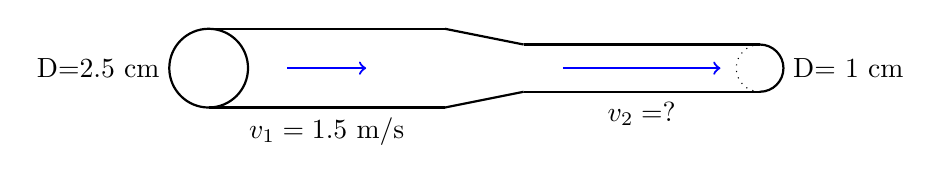
\begin{tikzpicture}
			
			% Large pipe section
			\draw[thick] (-3,0.5) -- (0,0.5);
			\draw[thick] (-3,-0.5) -- (0,-0.5)  node[midway, below] {$v_1 = 1.5$ m/s} ;
			\draw[thick] (-2.5,0) arc[start angle=0, end angle=360, radius=0.5];
			\node[left] at (-3.5,0) {D=2.5 cm};
			
			% Narrowing section
			\draw[thick] (0,0.5) -- (1,0.3);
			\draw[thick] (0,-0.5) -- (1,-0.3);
			
			% Small pipe section
			\draw[thick] (1,0.3) -- (4,0.3);
			\draw[thick] (1,-0.3) -- (4,-0.3)  node[midway, below] {$v_2 = ?$};
			\draw[thick] (4,0.3) arc[start angle=90, end angle=-90, radius=0.3];
			\draw[dotted] (4,0.3) arc[start angle=90, end angle=270, radius=0.3];
			\node[right] at (4.3,0) {D= 1 cm};
			
			% Velocity arrows
			\draw[->,thick,blue] (-2,0) -- (-1,0);
			\draw[->,thick,blue] (1.5,0) -- (3.5,0);
			
			% Water flow direction
		%	\draw[->,thick] (-3.5,0) -- (-3,0) node[left] {Water Flow};
			
		\end{tikzpicture}
		
	\vspace{0.1 in}
	
	In order to apply the continuity equation, we need to know the radius of each side.  Since we are given the diameter, $r_1 = \frac{\SI{2.5}{cm}}{2} = \SI{1.25}{cm}$ and $r_2 = \frac{\SI{1}{cm}}{2} = \SI{0.5}{cm}$.  We can now apply the continuity equation, seen above as equation \ref{equation:fluidcontinuity}.  Solving for $v_2$ yields:
	
	
	\begin{equation*}
		A_1 v_1 = A_2 v_2 \longrightarrow v_2 = \frac{A_1 v_1} {A_2}
	\end{equation*}
	Since both sides have a circular cross section, we can substitude $A=\pi r^2$.  
	
		\begin{equation*}
		v_2 = \frac{A_1 v_1} {A_2} = \frac{\cancel{\pi} {r_1}^2 v_1}{\cancel{\pi} {r_2}^2} = \frac{(\SI{1.25}{cm})^2(\SI{1.5}{m/s})}{(\SI{0.5}{cm})^2} \approx \SI{9.375}{m/s}
	\end{equation*}
	
\end{mdframed}
\vspace{0.1in}



\section{Bernouli's Equation}

Just as the continuity equation is derived from the law of conservation of mass, one can derive another equation from the law of conservation of energy.  This equation is named for Daniel Bernouli, who was the first to derive and publish it.

	\index{Bernouli's Equation}
				\begin{mdframed}[backgroundcolor=orange!20!white]
		\begin{equation}
			\rho g h_1 + \frac{1}{2} \rho v_1^2 + P_1 = \rho g h_2 + \frac{1}{2} \rho v_2^2 + P_2
			\label{equation:bernouli}
		\end{equation}
	\end{mdframed}	
While Bernouli's equation may look intimidating, one should always start by determining if there are equivilant terms on each side of the equation.  Equivalent terms on both side of the equation can be subtracted from both sides, making the equation significantly easier to solve.  



	\begin{mdframed}[backgroundcolor=blue!10!white]
	\begin{center}
		
		
		\textbf{Example \thesection.2}	
	\end{center}
	
	\textbf{Problem:}  
	Water flows through a horizontal pipe with a diameter of \SI{8}{cm} at a speed of \SI{3}{m/s}. The pipe then narrows to a \SI{3}{cm} diameter section. Assuming incompressible, non-viscous flow, what is the pressure difference between the wider and narrower sections of the pipe?
	
	\vspace{0.2in}
	
	\textbf{Solution:}   First, draw a diagram:
	
		\vspace{.1in}
	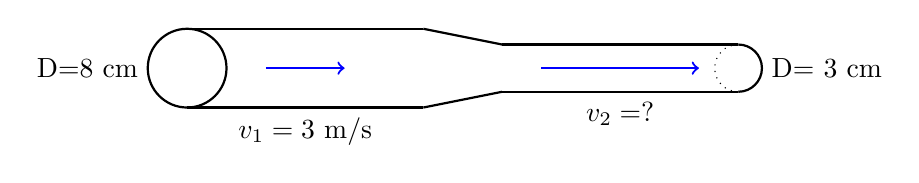
\begin{tikzpicture}
		
		% Large pipe section
		\draw[thick] (-3,0.5) -- (0,0.5);
		\draw[thick] (-3,-0.5) -- (0,-0.5)  node[midway, below] {$v_1 = 3$ m/s} ;
		\draw[thick] (-2.5,0) arc[start angle=0, end angle=360, radius=0.5];
		\node[left] at (-3.5,0) {D=8 cm};
		
		% Narrowing section
		\draw[thick] (0,0.5) -- (1,0.3);
		\draw[thick] (0,-0.5) -- (1,-0.3);
		
		% Small pipe section
		\draw[thick] (1,0.3) -- (4,0.3);
		\draw[thick] (1,-0.3) -- (4,-0.3)  node[midway, below] {$v_2 = ?$};
		\draw[thick] (4,0.3) arc[start angle=90, end angle=-90, radius=0.3];
		\draw[dotted] (4,0.3) arc[start angle=90, end angle=270, radius=0.3];
		\node[right] at (4.3,0) {D= 3 cm};
		
		% Velocity arrows
		\draw[->,thick,blue] (-2,0) -- (-1,0);
		\draw[->,thick,blue] (1.5,0) -- (3.5,0);
		
		% Water flow direction
		%	\draw[->,thick] (-3.5,0) -- (-3,0) node[left] {Water Flow};
		
	\end{tikzpicture}
	
	\vspace{0.1 in}
	
			
	\textbf{Step 1: Solve for \( v_2 \) using the continuity equation}  
	Since the flow is incompressible, we use the continuity equation:
	
	\begin{equation*}
		A_1 v_1 = A_2 v_2
	\end{equation*}
	
	where the cross-sectional area of a pipe is given by:
	
	\begin{equation*}
		A = \pi \left(\frac{d}{2} \right)^2.
	\end{equation*}
	
	Substituting for both pipe sections:
	
	\begin{equation*}
		\pi \left(\frac{d_1}{2} \right)^2 v_1 = \pi \left(\frac{d_2}{2} \right)^2 v_2.
	\end{equation*}
	
	Canceling \( \pi \) and solving for \( v_2 \):
	
	\begin{equation*}
		v_2 = v_1 \left( \frac{d_1}{d_2} \right)^2
	\end{equation*}
	
	Substituting \( d_1 = \SI{8}{cm} \) and \( d_2 = \SI{3}{cm} \):
	
	\begin{equation*}
		v_2 = (\SI{3}{m/s}) \left( \frac{\SI{8}{cm}}{\SI{3}{cm}} \right)^2  \approx 21.333 \text{ m/s}
	\end{equation*}
	

	
	\textbf{Step 2: Solve for \( P_1 - P_2 \) using Bernoulli’s equation}  
	
	We apply \textbf{Bernoulli’s equation} between the two sections of the pipe:
	
	\begin{equation*}
		 \rho g h_1 +  \frac{1}{2} \rho v_1^2 + P_1 =  \rho g h_2 + \frac{1}{2} \rho v_2^2 + P_2 
	\end{equation*}
	
	Since the pipe is horizontal, there is no change in the height of the pipe.  Therefore, the $rho g h$ can be subtracted from each side.
	
		\begin{equation*}
		\cancel{\rho g h_1} +  \frac{1}{2} \rho v_1^2 +  P_1 =  \cancel{\rho g h_2 }+ \frac{1}{2} \rho v_2^2 + P_2 
	\end{equation*}
	
	
	
	
	
	Rearranging Bernoulli’s equation:
	
	\begin{equation*}
		P_1 - P_2 = \frac{1}{2} \rho \left(v_2^2 - v_1^2 \right).
	\end{equation*}
	
	Substituting known values:
	
	\begin{equation*}
		P_1 - P_2 = \frac{1}{2} (1000) \left( 21.33^2 - 3^2 \right) \approx 2.23 \times 10^5 \text{ Pa}.
	\end{equation*}
	
	Thus, the pressure \textbf{decreases by} \( \mathbf{2.23 \times 10^5} \) \textbf{Pa} in the narrow section of the pipe.
	

	
\end{mdframed}
\vspace{0.1in}

